\subsection{Autocorrelazione e Autocorrelazione parziale}
In questa sezione verranno presentate le funzioni di autocorrelazione ed autocorrelazione
parziale utilizzate nell'analisi di serie temporali per poter trovare pattern e la correlazione
diretta o indiretta della serie con una sua versione spostata lungo l'asse temporale.

Nota che per molte applicazioni (come l'analisi di pattern) che utilizzano le funzioni
di autocorrelazione ed autocorrelazione parziale, le serie temporali devono essere stazionarie.

\subsubsection{Funzione di Autocorrelazione}
L'autocorrelazione definisce il grado di dipendenza tra i valori assunti 
da una funzione campionata nel suo dominio in ascissa. \\
Se è dimostrata l'autocorrelazione tra due valori, al cambiare delle peculiarità 
di uno di essi varierà anche l'altro.

L'autocorrelazione è uno strumento matematico usato frequentemente nella teoria dei 
segnali per l'analisi di funzioni o di serie di valori. Essa è la correlazione 
del segnale (o più in generale del valore di una variabile) con se stesso; 
in altre parole il segnale all'istante di tempo $t$ viene confrontato con un altro valore 
di se stesso ritardato di una quantità 
$\tau$  (senza tale ritardo il segnale è logicamente sempre uguale) 
per verificare quanto si somigli (più precisamente quanto si correli) 
all'avanzare del tempo. Possiamo dedurre che se un segnale varia lentamente nel tempo, 
il valore degli istanti $y(t)$ e $y(t + \tau)$ sarà pressoché simile 
(l'autocorrelazione avrà segno positivo), mentre se varia rapidamente, 
il valore di tali istanti sarà molto diverso e l'autocorrelazione assume 
un valore prossimo allo zero. 
L'autocorrelazione si utilizza spesso per cercare porzioni periodiche che si ripetono 
all'interno di un segnale, in modo tale da determinare la presenza di un segnale 
periodico che è stato sepolto da un rumore, o identificare la frequenza fondamentale 
di un segnale~\cite{wiki:autcor_it}.

Informalmente, è la somiglianza tra le osservazioni di una variabile casuale 
in funzione dell'intervallo di tempo che le separa~\cite{wiki:autcor_en}.

\paragraph{Definizione matematica} 
\subparagraph*{Caso continuo}
Dato un segnale $f(t)$ continuo ed indicizzato nel tempo, l'autocorrelazione $R_{ff}(\tau)$
è definita come la cross-correlazione di $f(t)$ con se stesso avente un ritardo di $\tau$
\[R_{ff}(\tau) = \int_{-\infty}^{\infty} f(t+\tau) \overline{f(t)}  \,dt =  \int_{-\infty}^{\infty} f(t) \overline{f(t-\tau)}  \,dt \]
dove $\overline{f(t)}$ indica il complesso coniugato fi $f(t)$. 
Nota come il parametro $t$ nell'integrale è una variabile fittizia ed è solo necessaria
a calcolare l'integrale. Non ha un significato specifico~\cite{wiki:autcor_en}.

\subparagraph*{Caso discreto}
Nel caso discreto la funzione di autocorrelazione è definita come:
\[ R_{ff}(\tau) = \mathbb{E} \left[ f(t) \overline{f(t-\tau)} \right] = \mathbb{E} \left[ f(t + \tau) \overline{f(t)} \right] \] 

\subparagraph*{Normalizzazione del caso discreto}
La normalizzazione della funzione di autocorrelazione nel caso discreto ci fornisce la 
possibilità di avere una visualizzazione con valori compresi tra $[-1, 1]$. 
Sottraendo la media prima della moltiplicazione si ottiene la funzione di autocovarianza 
\[ 
K_{ff}(\tau) = 
\mathbb{E} \left[ \left( f(t + \tau) - \mu \right) \overline{ \left( f(t) - \mu \right) } \right] =  
\mathbb{E} \left[ f(t + \tau) \overline{ f(t) } \right] - \mu\overline{\mu} 
\] 
dove $\mu$ è la media.


La funzione di autocorrelazione normalizzata viene definita come 

\[ 
\rho_{ff}(\tau) = \frac{K_{ff}(\tau)}{\sigma^2} = 
\frac{\mathbb{E} \left[ \left( f(t + \tau) - \mu \right) \overline{ \left( f(t) - \mu \right) } \right]}{\sigma^2}
\] 



\paragraph{Implementazione della funzione di autocorrelazione ed esempi}
Vediamo ora come poter implementare la funzione di autocorrelazione (normalizzata).
\subparagraph*{Snippet} (\textit{shift di una funzione})
\begin{minted}{python3}
def shift(X, n):
    """ Shifta di n periodi la funzione X
    """


    # controllo per n
    if not isinstance(n, int):
        raise Exception('n deve essere un valore intero')

    X_copy = X.copy() # copia e rendi numpy array
    if not isinstance(X_copy, np.ndarray):
        X_copy = np.array(X_copy)

    # se si shifta troppo impostiamo n
    # alla lunghezza della funzione X
    if np.abs(n) > len(X):
        n = np.sign(n) * len(X)
    
    # dato  n shiftiamo la funzione verso sinistra
    # dato -n shiftiamo la funzione verso destra
    for i in range(np.abs(n)):
        # togliamo il primo o lultimo valore
        # in base a dove vogliamo shiftare
        X_copy = X_copy[1:] if np.sign(n) == 1 else X_copy[:-1]

        # shifta la funzione aggiungendo uno 
        # 0 in testa o in coda in base a dove
        # vogliamo shiftare
        X_copy = np.insert(X_copy, 0 if np.sign(n) == -1 
            else len(X_copy), 0)

    return X_copy.tolist() if not isinstance(X, np.ndarray) \
        else np.array(X_copy)
\end{minted}

\subparagraph*{Snippet} (\textit{singola autocorrelazione})
\begin{minted}{python3}
    def singola_autocorrelazione(X: list | np.ndarray, 
    tau: int, normalizzazione = True) -> float:

    """ Esegue una signola autocorrelazione data la latenza
        tau
    """

    # controllo per tau
    if not isinstance(tau, int) and tau < 0:
        raise Exception('tau deve essere un intero \
            maggiore di 0')

    # controllo che X sia un array numpy
    if not isinstance(X, np.ndarray):
        X = np.array(X)


    if normalizzazione:
        mean = X.mean()
        var = X.var()
        
        # f(t-tau) - mu
        primo_termine   = shift(X - mean, -tau)

        # coniugato(f(t)- mu)
        secondo_termine = np.conjugate(X - mean)

        #                                           ... / sigma^2
        return np.mean( primo_termine * secondo_termine ) / var

    # espettazione[ f(t-tau)       * coniugato(f(t)) ]   
    return np.mean( shift(X, -tau) * np.conjugate(X) )
\end{minted}

\subparagraph*{Snippet} (\textit{funzione di autocorrelazione})
\begin{minted}{python3}
def funzione_autocorrelazione(
    X: list | np.ndarray,
    norm = True
    ) -> list | np.ndarray:
    
    """ calcola la funzione di autocorrelazione
    """
    autocorrelazione: list = []
    # calcola la autocorrelazione singola per ogni
    # possibile tau
    for i in range(len(X)):
        autocorrelazione.append(
            singola_autocorrelazione(X, i, 
                normalizzazione=norm)
        )

    return autocorrelazione if not isinstance(X, np.ndarray) \
        else np.array(autocorrelazione)
\end{minted}

\begin{esempio}[Autocorrelazione]
    Prendiamo come esepio un segnale la cui velocità cambia di ``poco''
    nel tempo.

    \begin{figure}[H]
        \centering
        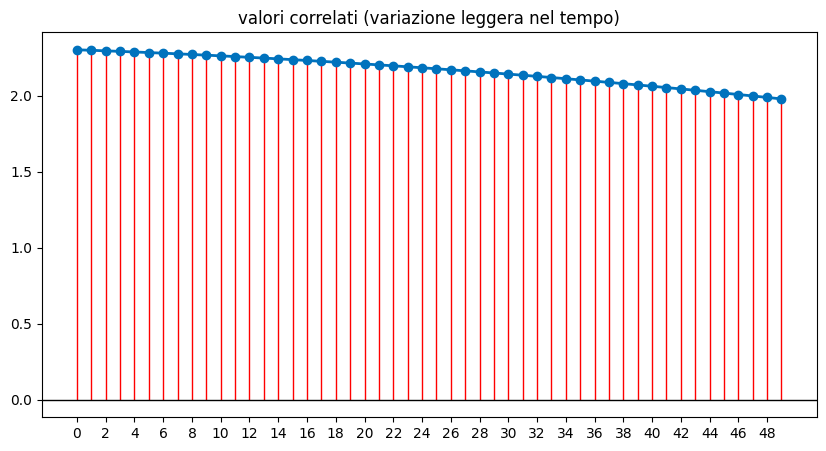
\includegraphics[width=0.9\linewidth,keepaspectratio]{autocor_vel_lenta.png}
        \caption{Autocorrelazione del segnale.}
        \label{fig:autcor_slow}
    \end{figure}

    In figura~\ref{fig:autcor_slow} possiamo notare come l'autocorrelazione non normalizzata
    del segnale varia di poco nel tempo per segnali che variano lentamente.

    Consideriamo ora più segnali la cui velocità cresce velocemente nel tempo.

    \begin{figure}[H]
        \centering
        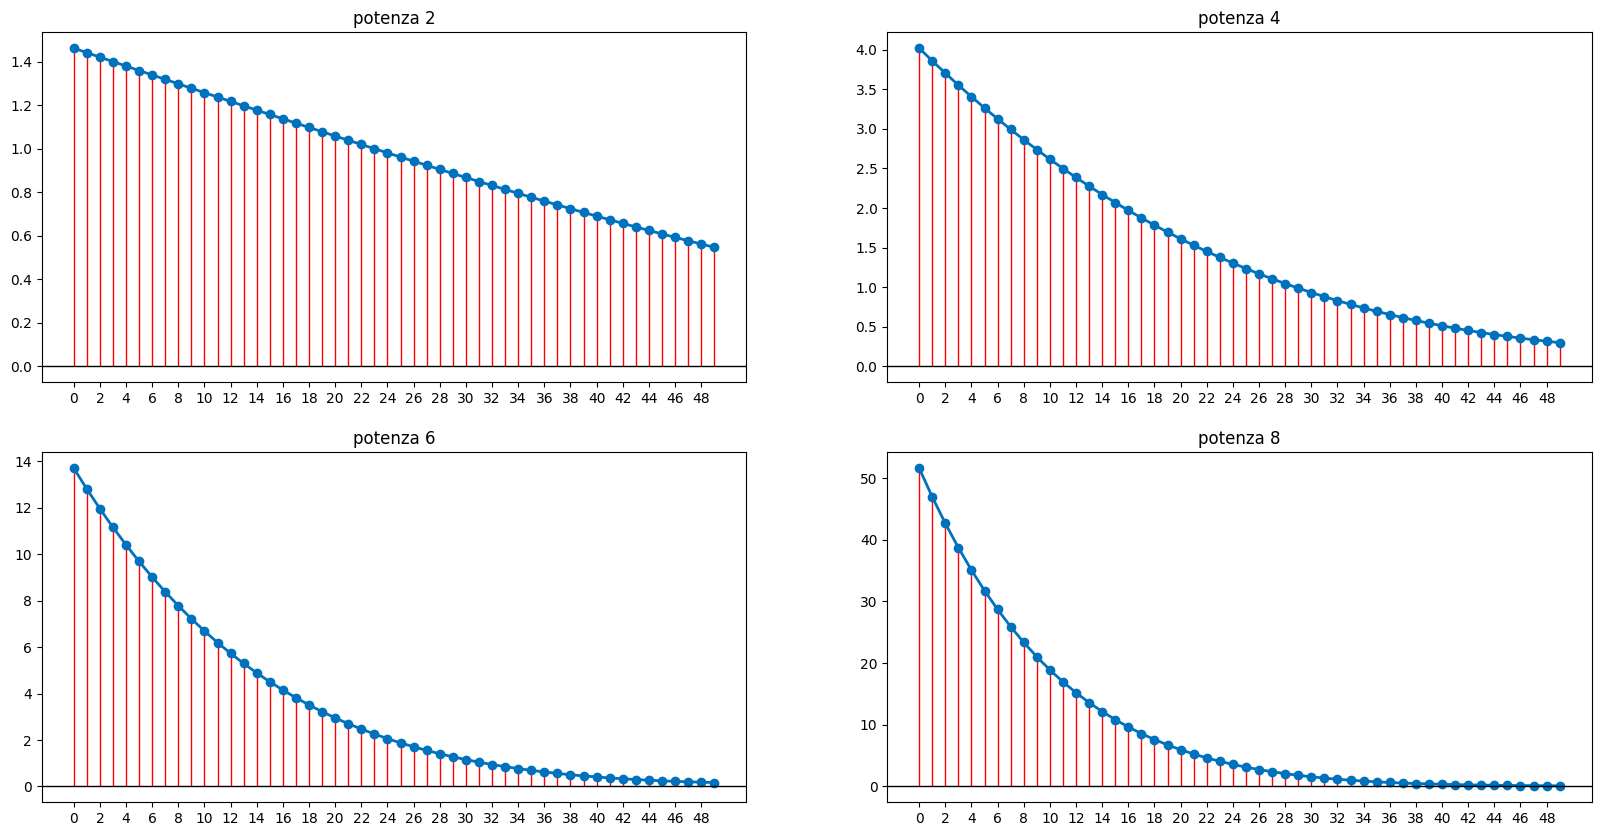
\includegraphics[width=\linewidth,height=9cm]{autocor_vel_fast.png}
        \caption{Autocorrelazione dei segnali.}
        \label{fig:autcor_fast}
    \end{figure}

    In figura~\ref{fig:autcor_fast} possiamo notare come l'autocorrelazione non normalizzata
    dei segnai varia maggiormente nel tempo per segnali che variano velocemente.

    Possiamo quindi osservare come segnali con minima variazione nel tempo avranno anche
    una minima variazione nell'autocorrelazione non normalizzata, mentre segnali che hanno
    un'ampia variazione tra un'osservazione e quella successiva avranno una maggiore variazione 
    anche nell'autocorrelazione non normalizzata.

    Un'ulteriore osservazione che nasce dagli esempi sopra è che i segnali più 
    correlati tra loro sono i segnali con una variazione minore nel tempo, mentre
    i segnali meno correlati saranno i segnali con una maggior variazione. 

\end{esempio}


\subsubsection{Funzione di Autocorrelazione Parziale}
L'autocorrelazione parziale, riassume la relazione tra 
un'osservazione di una serie temporale e le osservazioni di fasi temporali precedenti,
come la normale autocorrelazione con la diversità che le relazioni 
delle osservazioni intermedie vengono rimosse. In sostanza, 
le correlazioni indirette vengono eliminate lasciando visibile solamente
l'effetto diretto~\cite{md:mediumacf_pacf}.

Potreste, ad esempio, essere interessati alla relazione diretta tra i consumi 
di oggi e quelli di un anno fa. Non vi importa nulla di ciò che accade nel mezzo.

Il consumo dei 12 mesi precedenti ha un effetto sul consumo degli 11 mesi precedenti 
e il ciclo continua fino al periodo più recente. Nelle stime di autocorrelazione parziale, 
questi effetti indiretti vengono ignorati~\cite{ain:acf_pacf}.

\paragraph{Calcolo della funzione di autocorrelazione parziale}
La funzione di autocorrelazione parziale teorica di una serie temporale 
stazionaria può essere calcolata utilizzando l'algoritmo di Durbin-Levinson:
\[ \phi_{n,n} = 
\frac
{\rho(n) - \sum_{k = 1}^{n-1}  \phi_{n-1,k}\rho(n-k)}
{1 - \sum_{k = 1}^{n-1} \phi_{n-1,k}\rho(k)} 
\]
    
dove $\phi_{n,k} = \phi_{n-1,k} - \phi_{n,n}\phi_{n-1,n-k}$ per $1 \leq k \leq n-1$ and
$\rho(n)$ è la funzione di autocorrelazione~\cite{wiki:pacf}.

\paragraph{Quando è utile l'autocorrelazione parziale}
La funzione di autocorrelazione parziale gioca un ruolo molto importante, nell'analisi
di serie temporali, per l'identificazione dei lag ``importanti'' per un modello autoregressivo
(AR). Essendo che lo scopo del tirocinio è analizzare 
serie temporali senza eseguire nessuna predizione sui dati con modelli autoregressivi, non verrà
data un'iplementazione della formula presente sopra.

\paragraph{Pacchetto per l'utilizzo}
La funzione \texttt{pacf}, del modulo\\ \texttt{statsmodels.tsa.stattools}, e la funzione
\texttt{plot\_pacf}, del modulo\\ \texttt{statsmodels.graphics.tsaplots}, forniscono rispettivamente
un'implementazione della funzione di autocorrelazione parziale ed il grafico di essa.


